\documentclass[tikz,border=7pt]{standalone}
\usepackage{amsmath,amssymb}
\usepackage[scaled]{helvet}
\renewcommand{\familydefault}{\sfdefault}
\usetikzlibrary{arrows.meta,backgrounds,calc,fit,positioning,shapes.geometric}
\definecolor{bpink}{HTML}{172033}
\definecolor{bpblue}{HTML}{2A78D6}
\definecolor{bporange}{HTML}{E56A32}
\definecolor{bpgreen}{HTML}{168A65}
\definecolor{bppurple}{HTML}{7A5CC7}
\definecolor{bpred}{HTML}{C94A4A}
\definecolor{bpmuted}{HTML}{667085}
\definecolor{bpgrid}{HTML}{D8DEE8}
\definecolor{bpsurface}{HTML}{F8FAFC}
\tikzset{
  var/.style={circle,draw=bpblue,fill=bpblue!10,line width=.9pt,minimum size=8mm,font=\small\bfseries,text=bpink},
  factor/.style={rectangle,rounded corners=1.5pt,draw=bporange,fill=bporange!14,line width=.9pt,minimum size=6.8mm,font=\small\bfseries,text=bpink},
  constraint/.style={rectangle,rounded corners=1.5pt,draw=bpred,fill=bpred!12,line width=.9pt,minimum size=6.8mm,font=\small\bfseries,text=bpink},
  edge/.style={draw=bpmuted!75,line width=.9pt},
  msgvf/.style={-{Latex[length=2.2mm]},draw=bpblue,line width=1.35pt},
  msgfv/.style={-{Latex[length=2.2mm]},draw=bporange,line width=1.35pt},
  label/.style={font=\scriptsize,text=bpmuted,align=center},
  title/.style={font=\bfseries\large,text=bpink},
  card/.style={draw=bpgrid,fill=bpsurface,rounded corners=7pt,line width=.7pt},
}

\begin{document}
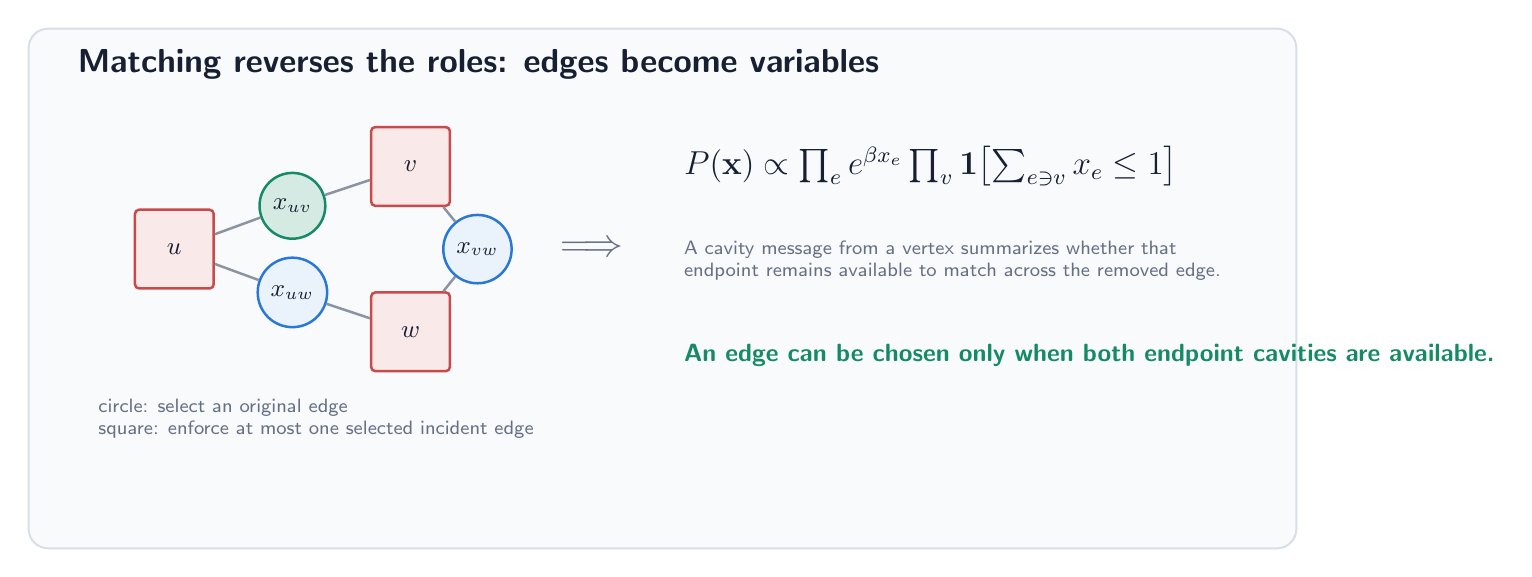
\begin{tikzpicture}[font=\sffamily]
  \node[card,minimum width=16.1cm,minimum height=6.6cm] at (7.2,2.0) {};
  \node[title,anchor=west] at (-.35,4.85) {Matching reverses the roles: edges become variables};
  \node[constraint,minimum size=10mm] (v1) at (1.0,2.5) {$u$};
  \node[constraint,minimum size=10mm] (v2) at (4.0,3.55) {$v$};
  \node[constraint,minimum size=10mm] (v3) at (4.0,1.45) {$w$};
  \node[var,fill=bpgreen!18,draw=bpgreen] (e12) at (2.5,3.05) {$x_{uv}$};
  \node[var] (e13) at (2.5,1.95) {$x_{uw}$};
  \node[var] (e23) at (4.85,2.5) {$x_{vw}$};
  \draw[edge] (v1)--(e12)--(v2) (v1)--(e13)--(v3) (v2)--(e23)--(v3);
  \node[label,align=left] at (2.8,.35) {circle: select an original edge\\square: enforce at most one selected incident edge};
  \node[text=bpmuted,font=\Large] at (6.3,2.5) {$\Longrightarrow$};
  \node[anchor=west,text=bpink,font=\large] at (7.35,3.55) {$P(\mathbf x)\propto\prod_e e^{\beta x_e}\prod_{v}\mathbf 1\!\left[\sum_{e\ni v}x_e\le1\right]$};
  \node[anchor=west,label,align=left] at (7.35,2.35) {A cavity message from a vertex summarizes whether that\\endpoint remains available to match across the removed edge.};
  \node[anchor=west,text=bpgreen,font=\small\bfseries] at (7.35,1.15) {An edge can be chosen only when both endpoint cavities are available.};
\end{tikzpicture}
\end{document}
